\chapter{Stato dell'Arte}
\label{chap:stato_arte}

\section{Tecnologie IoT}
L'Internet of Things (IoT) rappresenta una rete di dispositivi fisici, veicoli incorporati con elettronica, software, sensori e connettività di rete.
Questi dispositivi sono progettati per raccogliere e scambiare dati, consentodogli di comunicare con l'ambiente circostante.
Negli anni diverse tecnologie sono state usate per far comunicare questi dispositivi, la maggiorparte di queste si basano su radio frequenze, 
come LoRa, NB-IoT, ZigBee, Wi-Fi, BLE, fortemente indirizzate ad un uso outdoor o indoor. \\

Tuttavia, esistono scenari in cui la propagazione elettromagnetica incontra limiti
strutturali, ad esempio in ambienti sotterranei, gallerie, miniere o condotti, dove
l'attenuazione del segnale cresce a causa della composizione del terreno e
dell'umidità. In questi contesti, l'affidabilità della comunicazione wireless
tradizionale risulta fortemente compromessa.

\section{Comunicazione in ambienti sotterranei}
La comunicazione in ambienti sotterranei rappresenta una sfida significativa a causa delle caratteristiche uniche di questi ambienti.
Le onde elettromagnetiche, comunemente utilizzate per la comunicazione wireless, soffrono di attenuazioni elevate dovute alla permittività
del terreno e all'umidità, con una conseguente riduzione della portata e dell'affidabilità dei ponti radio \citep[sec.~2]{akyildiz2006}.\\
In letteratura è possibile individuare diverse soluzioni proposte per affrontare queste sfide, tra cui si riconoscono due linee principali di ricerca:
\begin{itemize}
    \item l'uso di radio frequenze molto basse (VLF), medie (MF)
          o più alte (UHF, SHF), adattate a condizioni specifiche;
    \item l'uso di onde acustiche, che sfruttano la propagazione meccanica del suono
          attraverso solidi e fluidi.
\end{itemize}
\subsection{Radio frequenze}
Le ricerche sulle onde elettromagnetiche in gallerie e miniere hanno mostrato
limiti significativi: la propagazione è fortemente influenzata dalla geometria degli
ambienti e dalle proprietà elettriche del mezzo.
Le ricerche effettuate sulle onde elettromagnetiche in gallerie e miniere 
mostrano limiti significativi riguardanti la propagazione, che risulta fortemente influenzata 
dalla geometria degli ambienti e dalle proprietà elettriche del mezzo.\\
Gli studi del U.S. National Institute for Occupational Safety and Health’s (NIOSH) Office of Mine Safety and Health Research (OMSHR)
\citep{jacksha2016}, avvenuti in seguito a crolli di alcune miniere di carbone
in U.S. nel 2006 hanno piantato le fondamenta per l'uso di one elettromagnetiche SHF/UHF in ambienti sotterranei.\\
Attraverso una serie di antenne direzionali dalla misura di 1.2 metri e ricevitori collocati prima in linea
retta ad una distanza crescente, e poi in presenza di curve a 30°, 60°, 90° e 180° in condotti sotterranei 
hanno dimostrato che, in condizioni ottimali, la copertura può raggiungere i 33 metri, ma la presenza di curve strette, biforcazioni
 o ostacoli riduce drasticamente la portata \citep[sec.~3]{jacksha2016};
 inoltre lo stesso fenomeno è stato osservato anche negli studi effettuati da Jeho Lee \citep[p.~59]{Lee2000_RadioWavePropagationTunnels}.

\begin{figure}[H]
    \centering
    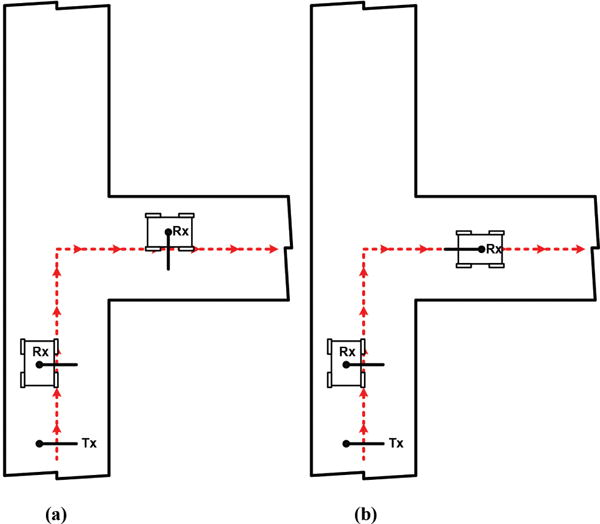
\includegraphics[width=0.30\textwidth]{immagini/corner_em.jpg}
    \caption{Mappa Tunnel U.S. National Institure for Occupational Safety and Health's\citep[sec.~3]{jacksha2016}.}
    \label{fig:esempio}
\end{figure}
Mentre
\citep[sec.~2]{akyildiz2006} descrivono le difficoltà intrinseche alla
propagazione sotterranea a causa di permittività e conducibilità elevate del terreno.\\

Più in generale, le tecnologie wireless pensate per ambienti sotterranei devono
fare i conti con una ridotta penetrazione delle frequenze tradizionalmente usate.\\
 Per questo, l'uso di frequenze estremamente basse (VLF, tra 3–30 kHz)
è stato studiato in scenari di emergenza e applicazioni militari, ma presenta
limiti di banda e di miniaturizzazione delle antenne \citep[sec.~5.1]{salam2023survey}.

\subsection{Onde acustiche}
Un'alternativa promettente alla comunicazione elettromagnetica in ambienti sotterranei è l'impiego di \emph{onde acustiche} (meccaniche), 
che si propagano attraverso solidi e fluidi (aria, acqua, fanghi di perforazione). A differenza delle onde EM, la propagazione acustica è 
spesso meno sensibile alla conducibilità elettrica del mezzo e può seguire percorsi guidati (ad es.\ lungo tubazioni o gallerie), con migliore 
resilienza a curve e biforcazioni \citep{fishta2023inpipe,heifetz2017pipes,farai2023mdpe}.

\paragraph{Modello di canale (cenni).}
Nei \textbf{solidi} (roccia, calcestruzzo, metalli, polimeri), la propagazione è dominata da onde elastiche (longitudinali e di taglio) e, in geometrie guidate 
(tubi, piastre, travi), da \emph{guided waves} (p.\,es.\ onde di Lamb o creep waves) con attenuazione che cresce fortemente con la frequenza e 
con il disaccoppiamento modale \citep[p.~2]{bianchi2023spazio}.\\ 
Nei \textbf{fluidi} in condotti (acqua/aria), il canale è tipicamente 
a bassa frequenza (centinaia di Hz–pochi kHz), con riflessioni multiple e dispersione; in vasche o condotti lunghi si osservano fenomeni di riverbero 
e frequenze di taglio dei modi guida \citep{fishta2023inpipe}. \\

\paragraph{Hardware e trasduttori.}
Sono impiegati trasduttori piezoelettrici o magnetostrittivi accoppiati meccanicamente al mezzo (collari su tubi, inserti su rocce/pareti, piastre di accoppiamento).\\
 Nei tubi metallici, coppie di attuatori/ricevitori permettono una comunicazione non invasiva (senza rompere il tubo), sfruttando onde di taglio o di Lamb 
 \citep[sec.~4.1]{heifetz2017pipes}.\\
Inoltre, per la comunicazione sotteranea si usano sorgenti e ricevitori acustici per mandare segnali nel terreno, 
fino a circa 50 m ma con velocità molto bassa (~20 bps) \cite[sec.~2.1]{yang2020soil}.\\

\paragraph{Tecniche di modulazione e codifica.}
Dato il canale fortemente dispersivo e soggetto a multi-percorso, si adottano modulazioni quali:
FSK/MFSK e BFSK a bassa frequenza creando collegamenti bassa velocità \citep{fishta2023inpipe,farai2023mdpe}.\\


\paragraph{Prestazioni riportate in letteratura.}
Risultati sperimentali rappresentativi includono:
\begin{itemize}
    \item \textbf{Suolo (through-soil).} Collegamenti fino a $\sim$50\,m con $\sim$20\,bps utilizzando portanti a bassa 
    frequenza e trasduttori compatti; dimostrazione di comunicazione digitale robusta in campi prova agricoli \citep[sec.~3]{yang2020soil}. 
    \item \textbf{Tubi metallici (acciaio).} Trasmissione di dati via onde elastiche lungo tubazioni esistenti in impianti industriali; 
    dimostrate immagini e pacchetti a centinaia di bps–pochi kbps su decine–centinaia di metri a bassa potenza, sfruttando onde di taglio
     e di Lamb \citep{heifetz2017pipes}.
    \item \textbf{Condotti idrici reali.} Revisione dei test in reti idriche urbane indica fattibilità di reti acustiche in-pipe per
     IoT, con vincoli di potenza, sincronizzazione e instradamento; lo stato dell’arte è pre-commerciale ma in rapida evoluzione \citep{fishta2023inpipe}.
\end{itemize}

\section{Applicazione della letteratura alla tesi}
La tesi si occuperà quindi della creazione di un protocollo di comunicazione acustica per sistemi distribuiti in ambienti sotteranei, 
basandosi sui risultati e le tecniche di cui sopra, è possibile quindi dedurre alcuni requisiti chiave:
Il protocollo opera nella banda 1–9 kHz, questa scelta è coerente con la letteratura, come visto nel \autoref{chap:introduzione}, 
inoltre l'utilizzo di una codifica FSK permetterà di avere un sistema robusto ma lento, coerentemente con le velocità di trasmissione viste in letteratura \citep{fishta2023inpipe}.\\
